\documentclass[11pt, a4paper]{article}
\usepackage[slovak]{babel}
\usepackage[utf8]{inputenc}

\usepackage{graphicx}
\usepackage{indentfirst}
\usepackage{cite}
\usepackage[table,xcdraw]{xcolor}

\author{Peter Schmiedt, Eduard Füzesséry}
\title{Lékařská informatika - Úloha zpracování a analýzy dat}

\graphicspath{{fig/}{logo/}}

\begin{document}

\begin{titlepage}
	\maketitle
\end{titlepage}



\section{Úvod}
Cieľom tejto úlohy je spracovanie a analýza dát z testovania účinnosti liečby dvoch rôznych liekov na primárnu chorobu a aký majú na to vplyv vek, BMI, sekundárne choroby, prítomnosť inej medikácie, atď.


Ďalšou úlohou je nájsť zaujímavé fakty a náväznosti medzi veličinami štatistickej významnosti.

\section{Spracovávané Dáta}



\begin{figure}[h!]
	\centering
  		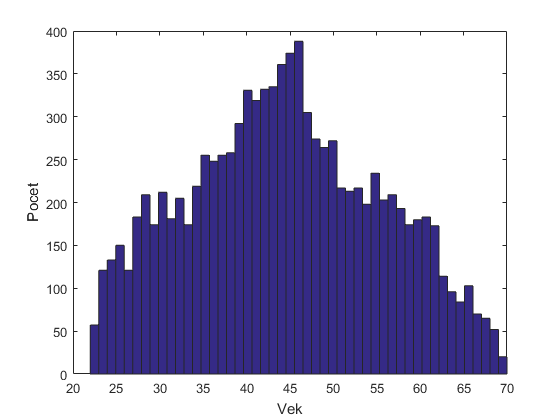
\includegraphics[width=1.0\textwidth]{ages.png}
  	\caption{Histogram Vekov}
\end{figure}

\section{Rozhodovací systém}

Prieniky jednotlivých kategórií si budeme značiť systémom ID, kde ID bude 4-ciferné číslo a každá cifra znamená nejakú konkrétnu kategóriu. Prvá cifra udáva vek, druhá cifra udáva MAP, tretia BMI a štvrtá cifra nám udáva prítomnosť inej medikácie počas liečby.

\begin{table}[!h]
\centering
\begin{tabular}{cc|
>{\columncolor[HTML]{38A4DA}}c 
>{\columncolor[HTML]{38A4DA}}c |
>{\columncolor[HTML]{F2BD35}}c 
>{\columncolor[HTML]{F2BD35}}c |
>{\columncolor[HTML]{32CB00}}c 
>{\columncolor[HTML]{32CB00}}c }
\hline
\textbf{Vek} & \textbf{}   & {\color[HTML]{333333} \textbf{MAP}} & {\color[HTML]{333333} \textbf{}}    & \textbf{BMI} & \textbf{} & \textbf{Prítomnosť inej medikácie} & \textbf{} \\ \hline
1000         & \textless30 & {\color[HTML]{333333} 100}          & {\color[HTML]{333333} \textless70}  & 10           & Podvýživa & Prítomná                           & 1         \\ \hline
2000         & 30-39       & {\color[HTML]{333333} 200}          & {\color[HTML]{333333} 70-92}        & 20           & Normál    & Neprítomná                         & 0         \\ \hline
3000         & 40-49       & {\color[HTML]{333333} 300}          & {\color[HTML]{333333} 93-105}       & 30           & Nadváha   &                                    &           \\ \hline
4000         & 50-59       & {\color[HTML]{333333} 400}          & {\color[HTML]{333333} 106-119}      & 40           & Obezita   &                                    &           \\ \hline
5000         & 60\textless & {\color[HTML]{333333} 500}          & {\color[HTML]{333333} 120\textless} &              &           &                                    &           \\ \hline
\end{tabular}
\caption{Rozhodovací systém}
\label{tab:rozhodovaci-system}
\end{table}

Napríklad: ID-2321 znamená že ide o pacientov vo veku 30-39 rokov, s MAP v rozsahu 93-105mmHg, BMI normálne a s prítomnosťou inej medikácie.

\section{Testovanie jednotlivých liekov}



\bibliography{literatura}{}
\bibliographystyle{plain}

\appendix
\section{Tabuľka účinnosti liekov}
\label{app:ucinnost-liekov}



\end{document}
